%%%%%%%%%%%%%%%%%%%%%%%%%%%%%%%%%%%%%%%%%%%%%%%%%%%%%%%%%%%%%%%%%%%%%%%%%%%%%%%%
%  Policy Evaluation Lab -- Lecture 6: Difference-in-differences
%  Oct 2026 restructuring: DiD as a design, not an estimator (one lecture
%  instead of two). Built from "lecture 7.tex" and "lecture 8.tex" (the PEL
%  versions of "lecture DID 1/2 - Matteo.tex", Public Policy Evaluation with
%  Migali). Kept: John Snow, parallel trends figures, Card and Krueger,
%  municipal unions. Dropped: NSW, Eissa-Liebman, Mariel, the derivations.
%  Sources checked for every number on the slides:
%   - Card and Krueger, NBER WP 4509 (1993) / AER 1994, Table 3: 23.33, 21.17,
%     20.44, 21.03, DiD 2.76 FTE (13 percent), t = 2.03; $4.25 -> $5.05 on
%     1 April 1992; 410 restaurants.
%   - Card and Krueger (2000, AER reply): payroll data figure (fig_kcdidtrend).
%   - Bronzini and de Blasio, March 2006 version (stored in materials/readings/
%     special-session-budget/papers): EUR 16 bn, 27,846 projects 1996-2003;
%     rejected applicants as controls; increase in the second year; slowdown
%     afterwards; CERVED 1993-2001.
%   - Ferraresi, Migali and Rizzo (2018, J. Regional Science): coefficients
%     -0.065 / -0.047 / -0.030 from the authors' table (tab_munion-didres).
%   - John Snow table: from the Migali deck; original tabulation not traced.
%%%%%%%%%%%%%%%%%%%%%%%%%%%%%%%%%%%%%%%%%%%%%%%%%%%%%%%%%%%%%%%%%%%%%%%%%%%%%%%%

\documentclass[aspectratio=169,xcolor=table]{beamer}
\input{preamble-pel}

\title[Policy Evaluation Lab]{Policy Evaluation Lab}
\subtitle[Lecture 6]{Lecture 6: Difference-in-differences}
\date[\pelYear]{October, 2026}

\newcolumntype{L}[1]{>{\raggedright\arraybackslash}p{#1}}
\begin{document}

\frame{\titlepage}

\begin{frame}{Where we are}
\small
\bi
  \item Lectures 4--5: when we can \textbf{randomise}, the comparison group is built for us
  \item Most policies are not randomised. This week and next: four designs that \textbf{find} a credible comparison group in existing data
\ei
\vspace{0.1cm}
\centering\footnotesize
\begin{tabular}{L{3.4cm}L{5.0cm}L{5.0cm}}
\toprule
\textbf{Design} & \textbf{The comparison group} & \textbf{Key assumption} \\
\midrule
Difference-in-differences & units not (yet) treated, over time & parallel trends \\
Regression discontinuity & units just below a cut-off & no sorting at the cut-off \\
Instrumental variables & units nudged by an outside factor & the factor works only through the treatment \\
Synthetic control & a weighted mix of untreated units & the mix tracked the treated unit before \\
\bottomrule
\end{tabular}
\pelTableNote{Today: the first row. We care about the logic and the assumption; the software does the arithmetic.}
\end{frame}

%%%%%%%%%%%%%%%%%%%%%%%%%%%%%%%%%%%%%%%%%%%%%%%%%%%%%%%%%%%%%%%%%%%%%%%%%%%%%%%%
\section{The idea}

\begin{frame}{From matching to differences}
\bi
  \item Back to our grant (Lecture 2): firms that apply are more motivated, better managed, more ambitious
  \item \textbf{Matching} compares each funded firm with a similar unfunded one, but only on what we \textbf{observe} (size, sector, age)
  \item Motivation and management are \textbf{not} in the data, so matching cannot remove them
\ei
\vspace{0.1cm}
\begin{block}{The difference-in-differences move}
If the unobserved differences between two groups are \textbf{constant over time}, comparing \textbf{changes} instead of \textbf{levels} cancels them out
\end{block}
\bi
  \item Two snapshots are not enough: we need each group \textbf{before and after} the policy
\ei
\end{frame}

\begin{frame}{The idea is old: John Snow and cholera}
\begin{columns}[T]
\begin{column}{0.44\textwidth}
\footnotesize
\bi
  \item London, 1850s: is cholera carried by air or by water?
  \item Two water companies served neighbouring houses from the Thames, downstream of the sewers
  \item In 1852 Lambeth moved its intake upstream; Southwark \& Vauxhall did not
  \item Snow compared the \textbf{change} in deaths between the 1849 and 1854 outbreaks
\ei
\end{column}
\begin{column}{0.54\textwidth}
\centering
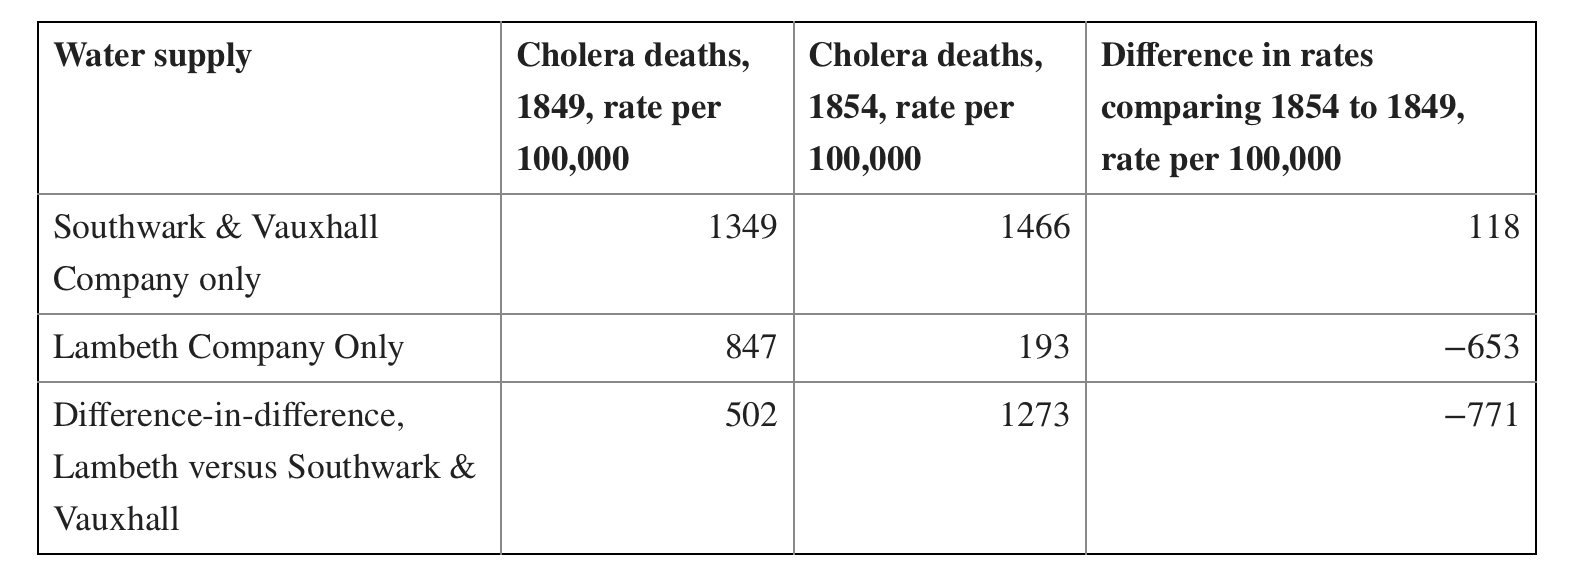
\includegraphics[width=\linewidth]{figures/lecture-06d/tab_jsnow-did.jpeg}
\pelTableNote{Cholera deaths per 100,000 people.}
\end{column}
\end{columns}
\end{frame}

\begin{frame}{Four numbers}
\centering
\begin{tabular}{lccc}
\toprule
 & \textbf{Before} & \textbf{After} & \textbf{Change} \\
\midrule
Treated  & $\bar Y_{T,\text{before}}$ & $\bar Y_{T,\text{after}}$ & $\Delta_T$ \\
Control  & $\bar Y_{C,\text{before}}$ & $\bar Y_{C,\text{after}}$ & $\Delta_C$ \\
\midrule
\multicolumn{3}{l}{\textbf{Difference-in-differences}} & $\Delta_T - \Delta_C$ \\
\bottomrule
\end{tabular}
\vspace{0.3cm}

\raggedright
\bi
  \item $\Delta_T$ alone (before--after) mixes the policy with everything else that changed at the same time
  \item Treated minus control \textbf{after} alone mixes the policy with permanent differences between the groups
  \item $\Delta_T - \Delta_C$ removes both, \textbf{if} the control group's change is what the treated would have experienced without the policy
\ei
\end{frame}

\begin{frame}{The picture}
\centering
\begin{tikzpicture}
\begin{axis}[pel chart, width=0.78\textwidth, height=0.66\textheight,
    xmin=0.6, xmax=2.4, xtick={1,2}, xticklabels={before, after},
    ymin=0, ymax=12, ytick=\empty, ylabel={outcome}, clip=false]
  \addplot[pelSlate, line width=1.3pt, mark=*] coordinates {(1,3) (2,5)};
  \addplot[pelAccent, line width=1.3pt, mark=*] coordinates {(1,6) (2,11)};
  \addplot[pelAccent, dashed, line width=1pt] coordinates {(1,6) (2,8)};
  \draw[pelText, <->, line width=0.8pt] (axis cs:2.08,8) -- (axis cs:2.08,11);
  \node[font=\footnotesize, text=pelText, anchor=west] at (axis cs:2.1,9.5) {effect};
  \node[font=\footnotesize, text=pelAccent, anchor=east] at (axis cs:0.95,6) {treated};
  \node[font=\footnotesize, text=pelSlate, anchor=east] at (axis cs:0.95,3) {control};
  \node[font=\scriptsize, text=pelAccent, anchor=north west] at (axis cs:1.35,6.7) {counterfactual: same change as control};
\end{axis}
\end{tikzpicture}
\pelTableNote{Illustrative numbers. The gap at the start does not matter; what matters is that, without the policy, the two lines would have moved together.}
\end{frame}

%%%%%%%%%%%%%%%%%%%%%%%%%%%%%%%%%%%%%%%%%%%%%%%%%%%%%%%%%%%%%%%%%%%%%%%%%%%%%%%%
\section{Parallel trends}

\begin{frame}{The one assumption that matters}
\small
\begin{block}{Parallel trends}
Without the policy, the outcome of the treated group would have changed by the same amount as that of the control group
\end{block}
\bi
  \item It is about the \textbf{counterfactual}, so it can never be tested directly
  \item The groups can differ in \textbf{levels}; they must not differ in \textbf{trends}
  \item It fails when something else hits one group at the same time, or when the groups were already drifting apart
\ei
\begin{exampleblock}{What we can do}
Look at \textbf{several years before} the policy. If the two groups moved together then, parallel trends after is more believable (not proven)
\end{exampleblock}
\end{frame}

\begin{frame}{Checking the years before}
\centering
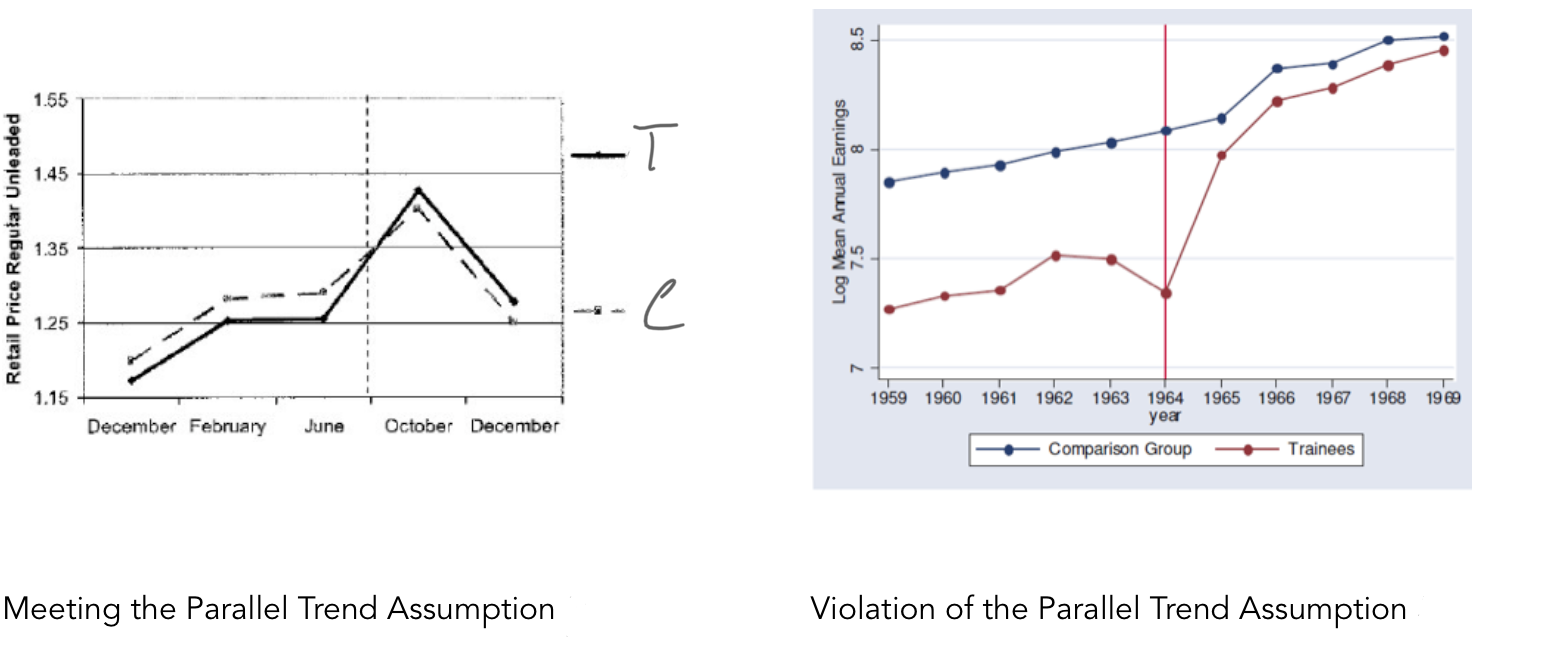
\includegraphics[height=0.64\textheight]{figures/lecture-06d/fig_did-partrendsex.jpeg}
\pelTableNote{With many periods we can plot the gap between the groups year by year: an \textbf{event study}. Flat before the policy, moving after: that is the pattern we hope for.}
\end{frame}

%%%%%%%%%%%%%%%%%%%%%%%%%%%%%%%%%%%%%%%%%%%%%%%%%%%%%%%%%%%%%%%%%%%%%%%%%%%%%%%%
\section{A classic: the minimum wage}

\begin{frame}{Card and Krueger (1994): does a higher minimum wage cost jobs?}
\small
\bi
  \item Textbook prediction: in a competitive market, a higher minimum wage reduces employment
  \item With employer market power, it need not: an empirical question
  \item \textbf{1 April 1992}: New Jersey raises its minimum wage from \$4.25 to \$5.05; neighbouring \textbf{Pennsylvania} does not
  \item Survey of \textbf{410 fast-food restaurants} in both states, before (Feb--Mar 1992) and after (Nov--Dec 1992)
\ei
\begin{exampleblock}{Why fast food?}
Many minimum-wage workers, similar products and jobs across chains, no tips: restaurants on the two sides of the border are comparable
\end{exampleblock}
\end{frame}

\begin{frame}{The result}
\begin{columns}[T]
\begin{column}{0.52\textwidth}
\centering
\small
\begin{tabular}{lccc}
\toprule
\textbf{FTE per store} & \textbf{PA} & \textbf{NJ} & \textbf{NJ -- PA} \\
\midrule
Before & 23.33 & 20.44 & $-2.89$ \\
After  & 21.17 & 21.03 & $-0.14$ \\
\midrule
Change & $-2.16$ & $0.59$ & \textbf{2.76} \\
\bottomrule
\end{tabular}
\pelTableNote{FTE = full-time equivalent employees. Card and Krueger (1994), Table 3, row 1--3.}
\end{column}
\begin{column}{0.45\textwidth}
\small
\bi
  \item New Jersey stores were \textbf{smaller} to begin with: levels differ, and that is fine
  \item Employment fell in Pennsylvania and rose slightly in New Jersey
  \item DiD: \textbf{+2.76} employees per store (about 13\%), significant at 5\%
  \item The opposite of the textbook prediction
\ei
\end{column}
\end{columns}
\end{frame}

\begin{frame}{Was Pennsylvania a good counterfactual?}
\begin{columns}[T]
\begin{column}{0.48\textwidth}
\centering
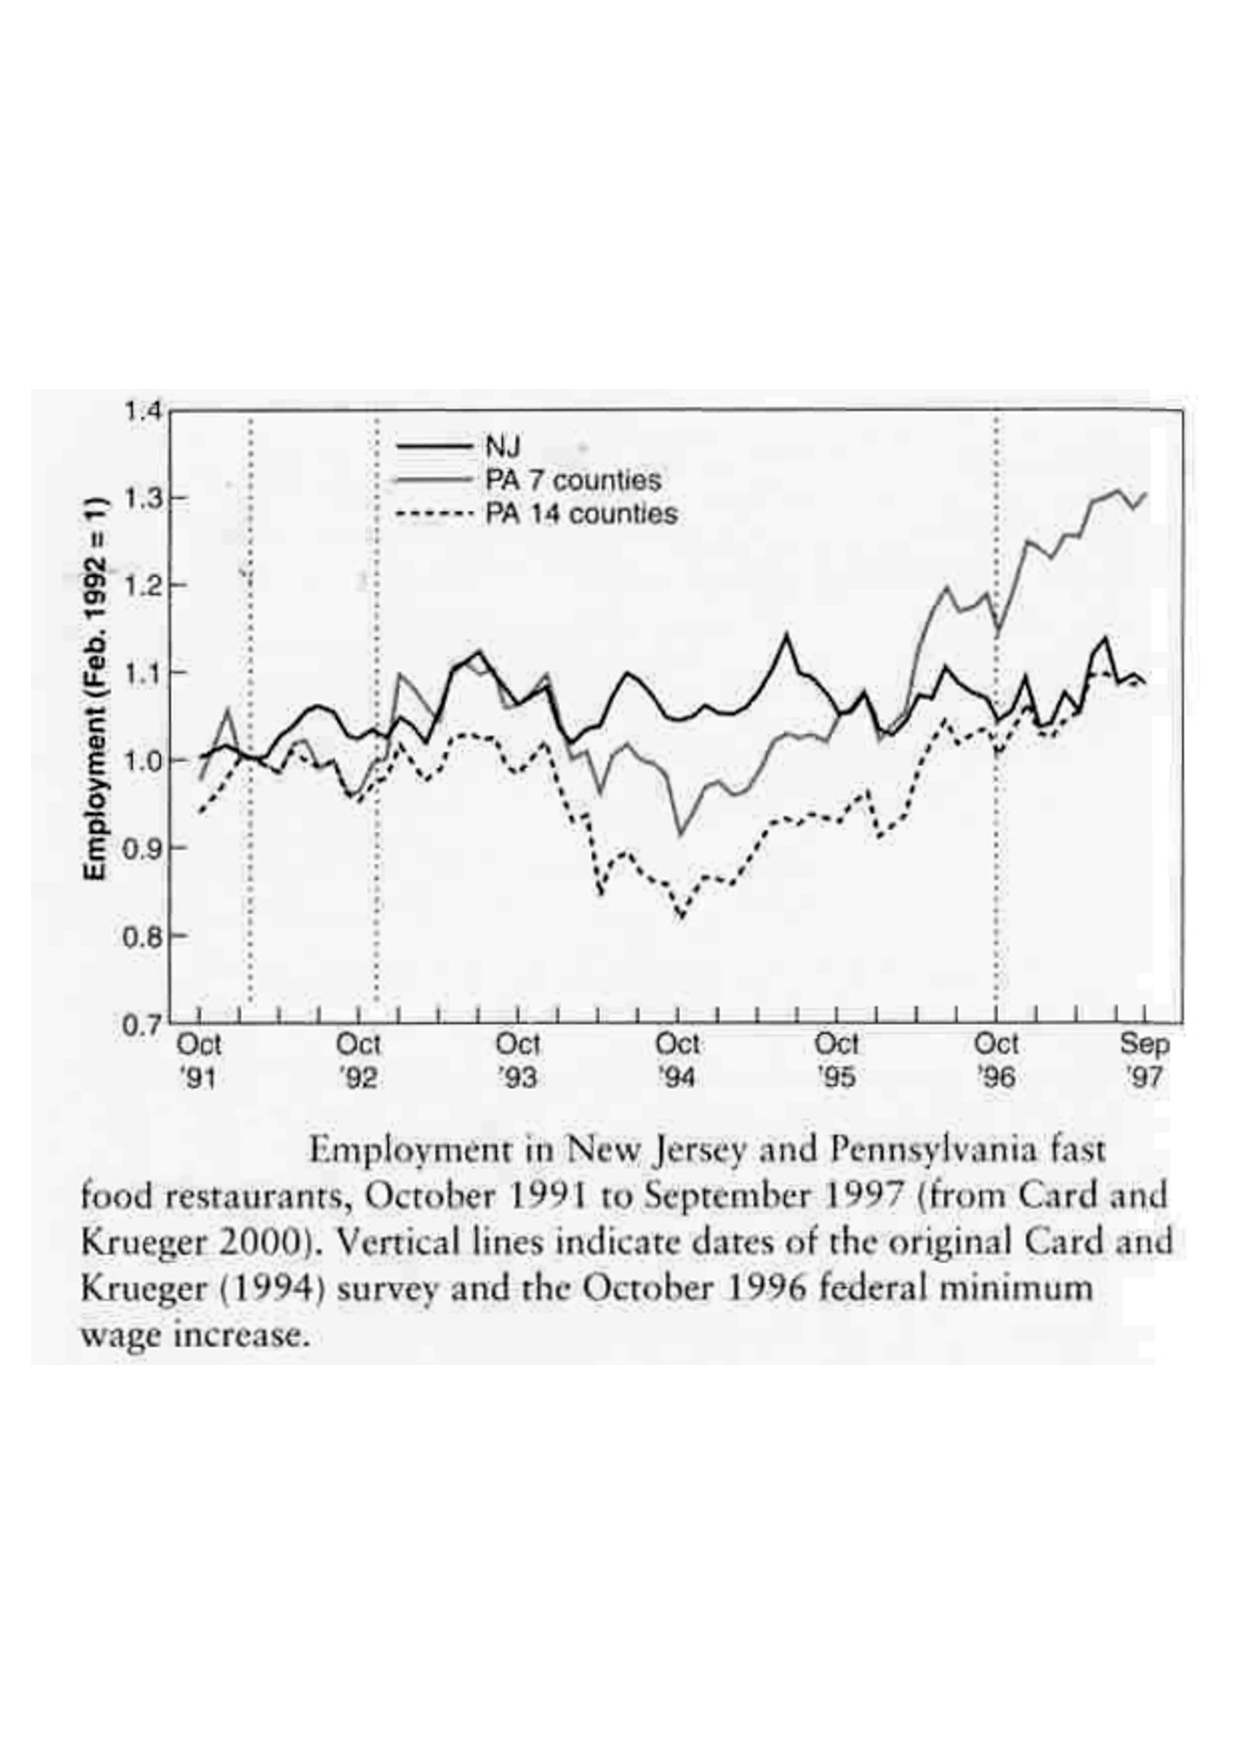
\includegraphics[width=\linewidth, trim=30 318 15 175, clip]{figures/lecture-06d/fig_kcdidtrend.pdf}
\end{column}
\begin{column}{0.5\textwidth}
\small
\bi
  \item With two survey waves we cannot see trends
  \item Later payroll data (Card and Krueger, 2000) cover 1991--1997
  \item Around the 1992 surveys the series move together; afterwards, employment in parts of Pennsylvania falls for years while the minimum wage is unchanged
  \item The debate on this study lasted years: it is a debate about \textbf{parallel trends}, not about the arithmetic
\ei
\end{column}
\end{columns}
\pelTableNote{Vertical lines: the two original surveys (1992) and the October 1996 federal increase.}
\end{frame}

%%%%%%%%%%%%%%%%%%%%%%%%%%%%%%%%%%%%%%%%%%%%%%%%%%%%%%%%%%%%%%%%%%%%%%%%%%%%%%%%
\section{Firms as targets: Law 488}

\begin{frame}{Law 488/1992: capital grants for the South}
\footnotesize
\bi
  \item For years the main Italian instrument against territorial gaps: 1996--2003, \textbf{€16 billion} to industrial firms, 27,846 projects, mainly in southern regions
  \item Firms apply, are \textbf{ranked} on pre-set criteria, and are funded from the top until the regional budget runs out
  \item Question: did the grants create investment that would not have happened otherwise?
\ei
\vspace{0.1cm}
\begin{block}{Bronzini and de Blasio (2006): the design}
\bi
  \item \textbf{Treated}: funded firms. \textbf{Control}: firms that applied but ranked too low
  \item Rejected applicants wanted to invest too: closer to funded firms than non-applicants (Lecture 2)
  \item Ministry files linked to financial statements, 1993--2001: years before \textbf{and} after
\ei
\end{block}
\end{frame}

\begin{frame}{What they found, and why it matters for policy}
\small
\bi
  \item Funded firms \textbf{increased investment}, mainly in the second year of the grant
  \item In the following years their investment \textbf{slowed down} relative to rejected firms
  \item Interpretation: part of the subsidised investment was \textbf{brought forward} from later years, not created
\ei
\vspace{0.15cm}
\begin{exampleblock}{The policy lesson}
A before--after comparison, or a look at the grant years only, would have overstated the effect. The control group \textbf{and} the years after the programme changed the conclusion
\end{exampleblock}
\pelTableNote{Thursday: the same ranking allows a second design, regression discontinuity (Cerqua and Pellegrini, 2014, reach a more positive conclusion).}
\end{frame}

%%%%%%%%%%%%%%%%%%%%%%%%%%%%%%%%%%%%%%%%%%%%%%%%%%%%%%%%%%%%%%%%%%%%%%%%%%%%%%%%
\section{Staggered adoption}

\begin{frame}{When units are treated at different times}
\small
\bi
  \item Policies often roll out gradually: regions, branches, municipalities join in different years
  \item Each year we compare units that have just joined with units that have not (yet)
\ei
\[ Y_{it} = \underbrace{\mu_i}_{\text{unit}} + \underbrace{\tau_t}_{\text{year}} + \gamma\, D_{it} + \varepsilon_{it} \]
$\mu_i$: permanent differences between units; $\tau_t$: shocks common to all in a year; $\gamma$: the DiD effect
\begin{alertblock}{A warning}
If the effect grows or fades over time, this regression can use early adopters as controls for late ones. Newer methods compare only with not-yet-treated units (Goodman-Bacon, 2021)
\end{alertblock}
\end{frame}

\begin{frame}{Municipal unions in Emilia-Romagna}
\begin{columns}[T]
\begin{column}{0.5\textwidth}
\small
\bi
  \item Ferraresi, Migali and Rizzo (2018): do small municipalities save money by sharing services in a \textbf{union}?
  \item Emilia-Romagna, 2001--2011; municipalities join unions in different years
  \item Outcome: current spending per inhabitant
\ei
\end{column}
\begin{column}{0.48\textwidth}
\centering
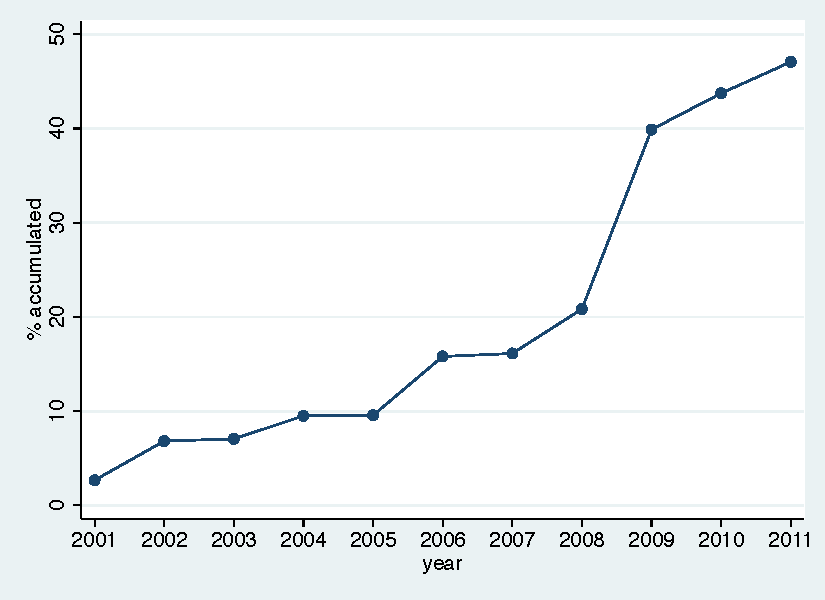
\includegraphics[height=0.62\textheight]{figures/lecture-06d/graph3.pdf}
\pelTableNote{Share of municipalities in a union.}
\end{column}
\end{columns}
\end{frame}

\begin{frame}{Municipal unions: results}
\begin{columns}[T]
\begin{column}{0.55\textwidth}
\centering
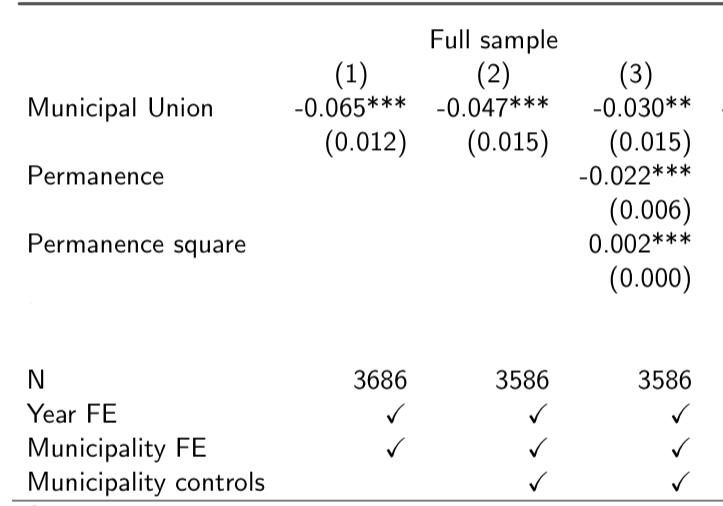
\includegraphics[width=0.88\linewidth]{figures/lecture-06d/tab_munion-didres.jpeg}
\end{column}
\begin{column}{0.42\textwidth}
\small
\bi
  \item Joining a union lowers current spending per inhabitant by about \textbf{3 to 6\%}, depending on the controls
  \item The estimate shrinks with more controls: what else differs between joiners and non-joiners?
  \item Efficiency or fewer services? The authors argue services did not fall; another study of Italian unions finds no clear effect (Luca and Modrego, 2021)
\ei
\end{column}
\end{columns}
\pelTableNote{Coefficients on log spending; municipality and year fixed effects in all columns.}
\end{frame}

%%%%%%%%%%%%%%%%%%%%%%%%%%%%%%%%%%%%%%%%%%%%%%%%%%%%%%%%%%%%%%%%%%%%%%%%%%%%%%%%
\section{Reading a DiD study}

\begin{frame}{Five questions to ask any DiD study}
\be
  \item \textbf{Who is the control group}, and why would it have followed the same path?
  \item Are there \textbf{several years before} the policy, and do the groups move together in them?
  \item Did anything \textbf{else} hit the treated group at the same time (another reform, a local shock)?
  \item Did the policy change \textbf{who is in} the groups (firms moving, closing, entering)?
  \item Do the results survive a \textbf{different control group} or a different period?
\ee
\vspace{0.1cm}
\begin{block}{}
\centering Strength: credible effects from data that already exist. Weakness: everything rests on one assumption about a path we never observe
\end{block}
\end{frame}

\begin{frame}{Friday lab and readings}
\bi
  \item \textbf{Friday}: two studies side by side (Card and Krueger; Bronzini and de Blasio). For each: the five questions, then what a policymaker should take from it
  \item Readings on the Lectures page, week 4
\ei
\vspace{0.15cm}
\begin{exampleblock}{Thursday}
Regression discontinuity: what a funding cut-off can tell us about R\&D grants
\end{exampleblock}
\end{frame}

\begin{frame}{References}
\tiny
\bi
  \item Bronzini, R. and G. de Blasio (2006), Evaluating the impact of investment incentives: the case of Italy's Law 488/1992, \textit{Journal of Urban Economics}, 60(2), 327--349
  \item Card, D. and A. B. Krueger (1994), Minimum wages and employment: a case study of the fast-food industry in New Jersey and Pennsylvania, \textit{American Economic Review}, 84(4), 772--793
  \item Card, D. and A. B. Krueger (2000), Minimum wages and employment: a case study of the fast-food industry in New Jersey and Pennsylvania: reply, \textit{American Economic Review}, 90(5), 1397--1420
  \item Cerqua, A. and G. Pellegrini (2014), Do subsidies to private capital boost firms' growth? A multiple regression discontinuity design approach, \textit{Journal of Public Economics}, 109, 114--126
  \item Ferraresi, M., G. Migali and L. Rizzo (2018), Does intermunicipal cooperation promote efficiency gains? Evidence from Italian municipal unions, \textit{Journal of Regional Science}, 58(5), 1017--1044
  \item Luca, D. and F. Modrego (2021), Stronger together? Assessing the causal effect of inter-municipal cooperation on the efficiency of small Italian municipalities, \textit{Journal of Regional Science}, 61(1), 261--293
  \item Goodman-Bacon, A. (2021), Difference-in-differences with variation in treatment timing, \textit{Journal of Econometrics}, 225(2), 254--277
  \item Snow, J. (1855), \textit{On the Mode of Communication of Cholera}, 2nd edition, London: John Churchill
\ei
\end{frame}

\pelQuestions

\end{document}
